\documentclass[class=article,crop=false]{standalone}

\usepackage{../setting/preamble_}

\begin{document}
\twocolumn

\section{Theory}
\subsection{Oscillator}
\begin{wrapfigure}{l}{0.3\columnwidth}
  \vspace*{-.5cm}
  \begin{center}
    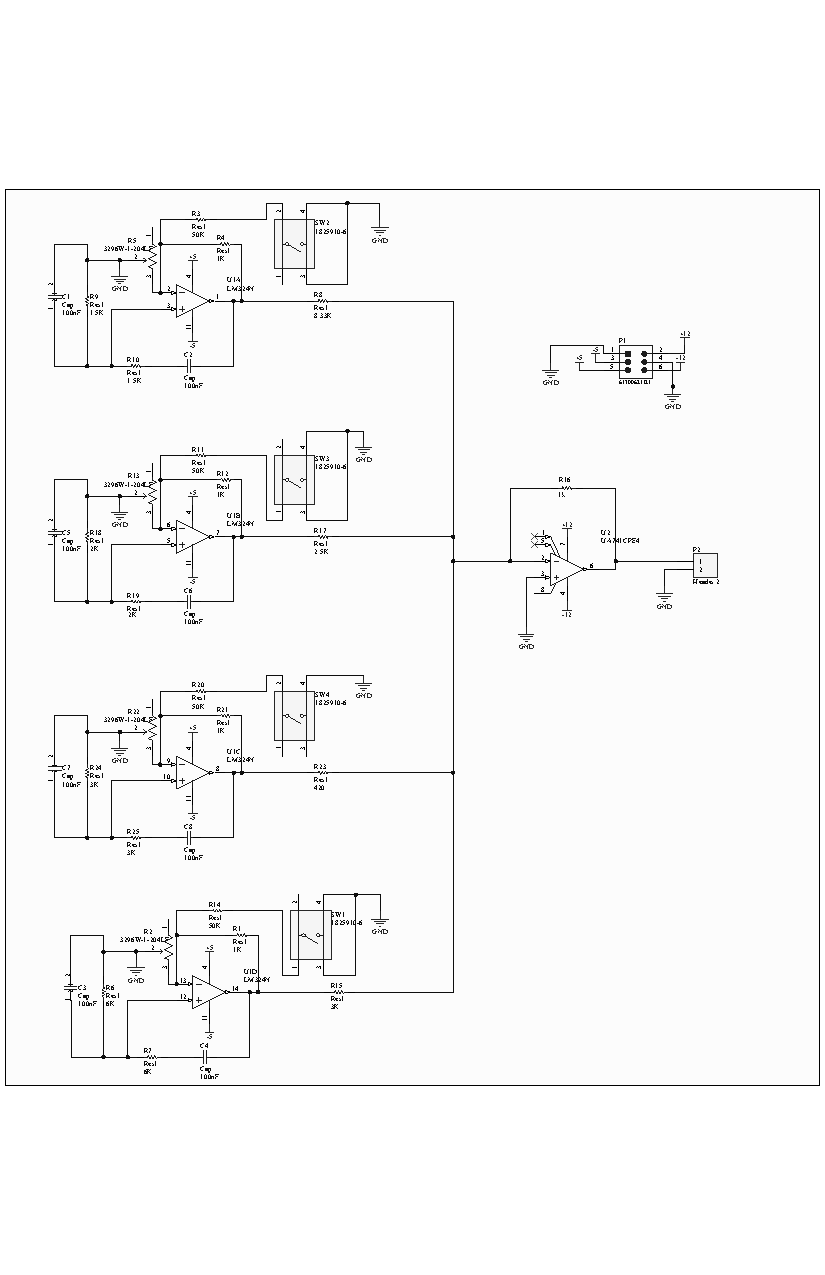
\includegraphics[width=0.3\columnwidth]{oscillator}
  \end{center}
  \vspace*{-.5cm}
\end{wrapfigure}

An oscillator is an amplifier that uses positive feedback that generates an output frequency without the use of an externally applied input signal. Once the oscillation is started, the parameters A and $\beta$ are aligned to maintain a unity gain at the required frequency in order to keep the oscillation indefinitely stable.

\subsubsection*{Wein-Bridge Oscillator}
The Wien Bridge Oscillator uses a feedback circuit consisting of a series RC node cascaded with a parallel RC of the same component values producing a phase delay or phase advance circuit depending upon the frequency. Effectively they act as a second-order frequency dependant Band-Pass-Filter with a high Q factor at the selected frequency $f_r=\frac{1}{2\pi RC}$. This RC network is connected in the positive feed-back path of the amplifier and has zero phase shift at just one frequency.
\par
Other part of the feedback signal is connected to the inverting input terminal(negative feed-back) via resistor divider network of $R_1\&R_2$.Then at the selected resonant frequency($f_r$), the voltages applied to the inverting and non-inverting inputs will be equal and “in-phase”. So the positive feedback will cancel out the negative feedback signal causing the circuit to oscillate.

\begin{figure} 
  \begin{subfigure}{.33\columnwidth}
    \centering
    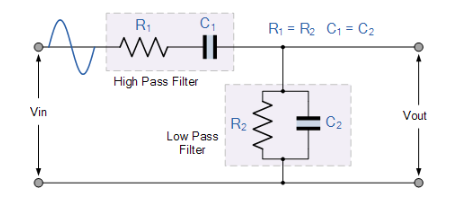
\includegraphics[width=.95\columnwidth]{weistan_1}
    \caption*{RC-Network}  
  \end{subfigure}
  \begin{subfigure}{.33\columnwidth}
    \centering
    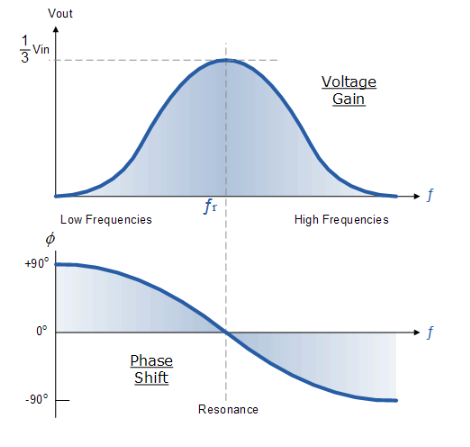
\includegraphics[width=.95\columnwidth]{weistan_2}  
    \caption*{Response}
  \end{subfigure}
  \begin{subfigure}{.3\columnwidth}
    \centering
    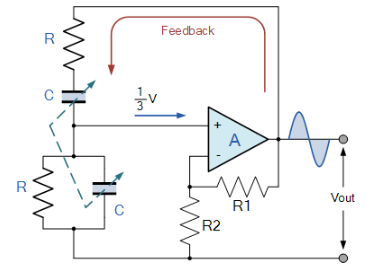
\includegraphics[width=.95\columnwidth]{weistan_3}
    \caption*{Oscillator}  
  \end{subfigure}
\end{figure}
\subsubsection*{Starting and Damping Oscillation}
By controlling the negative feedback ratio($\frac{R_2}{R_1+R_2}$) of the oscillator we can start and damp the oscillation as required. To start oscillation, we need to slightly reduce the negative feedback($<\frac{1}{3}$). This will give rise to a resultant signal on the amplifier input side which is get amplified and fed back recursively turns out to drive oscillation.
\par
Keeping the feedback ratio slightly more($>\frac{1}{3}$) will give rise to a resultant negative input which is get added adversely with output resulting in damping of the oscillation. By fine-tuning the ratio in a very elegant manner, it is possible to control the damping time constant.
\subsection{Amplifier}
Driving a high-power speaker draws a high amount of current from the circuit. These current ranges are very much higher than the maximum supply available from op-amps and other low power components used in generating the wave patterns. So it is crucial to maintain an amplifier boundary between low power noisy signal to high power driving signal free of noise. In the following context, we will discuss the theories behind our amplifier design in detail.
\subsubsection*{Class-A }
\begin{wrapfigure}{l}{0.35\columnwidth}
  \vspace*{-.5cm}
  \begin{center}
    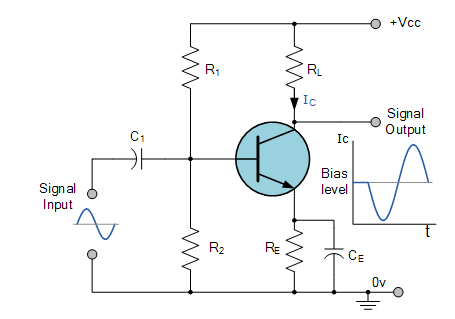
\includegraphics[width=0.35\columnwidth]{classA}
  \end{center}
  \vspace*{-.5cm}
\end{wrapfigure}
These are the simplest configuration among other families. It uses a single-ended transistor for its output stage with the resistive load connected directly to the Collector terminal. When the transistor switches “ON” it sinks the output current through the Collector resulting in an inevitable voltage drop across the Emitter resistance thereby limiting the negative output capability.  
\par 
The current handling capability of such an amplifier family can be increased drastically by replacing the output transistor with \textbf{Darlington pair}. These devices provide high input impedance.
\subsubsection*{Class-B}
Class B Amplifiers are biased to only conduct half of the input signal. Using 2 such amplifiers arranged in a “Push-Pull” configuration, and combining the output signal, the full waveform can be obtained.
\par
As the quiescent current for this amplifier is 0, there is little or no DC, therefore much less power dissipation. However, there is a slight waveform distortion due to the bias voltage requirement of the transistor known as cross-over distortion.
\subsubsection*{Class-AB} 
Class AB amplifiers overcome the distortion issue of class B amplifiers by permanently bringing the two transistors just into the active region. This reduces the efficiency, but results in an undistorted the waveform in the output.
\par
\begin{figure}
  \vspace*{-.7cm}
  \begin{center}
    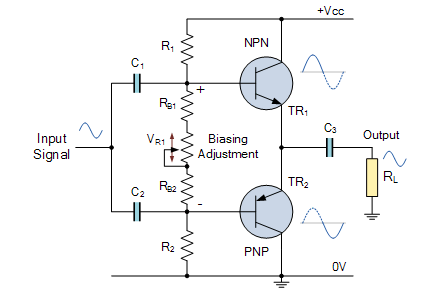
\includegraphics[width=.6\columnwidth]{classAB}
  \end{center}
  \vspace*{-.5cm}
\end{figure}
As the power dissipation due to the DC component is much less than class A amplifiers, these circuits allow the use of compact heat sinks during the operation.
\subsubsection*{Variable Zerner Diode}
\begin{wrapfigure}{r}{0.2\columnwidth}
  \vspace*{-1cm}
  \begin{center}
    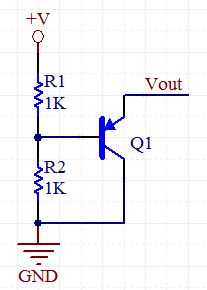
\includegraphics[width=0.2\columnwidth]{zener}
  \end{center}
  \vspace*{-.5cm}
\end{wrapfigure}
This variable Zener diode circuit acts like a Zener diode with a breakdown voltage adjustable in a vast domain. This is achieved by driving a BJT in the active region and controlling the base current. The current through the voltage divider $R_1\&R_2$ must be higher compared to the base current.
\end{document}